\chapter{Reinforcement Learning}
\textbf{Reinforcement Learning} came to the stage when the system developed by Google Deep-Mind \textbf{AlphaGo}. It has been shown that the best player of the game Go on the earth was beaten from the machine.

We have already discussed supervised and unsupervised learning, now the last machine learning area we need to talk about is the reinforcement learning.

As we have seen, in unsupervised learning we don't have access to any annotations at all for our data, and we've seen methods for clustering, dimensionality reduction, and density estimation. When have talked about supervised learning, we have seen methods for classification and regression, such as Neural Networks, SVM, \(k\)-NN, and so on...

We are now into the introduction to the Reinforcement Learning area, that has a completely different scheme of training, where the learning follows an iterative manner.

\section{The Idea}
The idea of reinforcement learning is inspired by the way in which human and animals learns. In this kind of learning, the problems involve an \textbf{agent} interacting with an \textbf{environment}, which provides numeric rewards signals.

The goal in reinforcement learning is to learn how to take actions in order to maximize the reward.

\begin{figure}[t!]
    \centering
    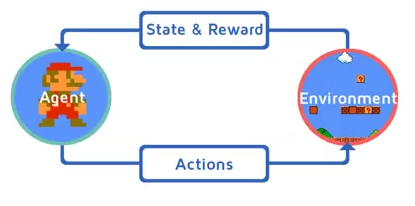
\includegraphics[width=.75\textwidth]{089}
    \caption{}
    \label{fig:089}
\end{figure}

Let's for example examine the Super Mario game, in this case the environment is the screen of the game, that can be described as the state \(s_t\); our agent for this example is Mario, that takes an action \(a_t\), \(a_t\) has in impact on the next state of the environment. Depending on the action Mario has made, he will take a negative or postiive reward \(r_t\), then we move to the next state \(s_{t+1}\), and the loop continues until the episode is finished.

\begin{figure}[h!]
    \centering
    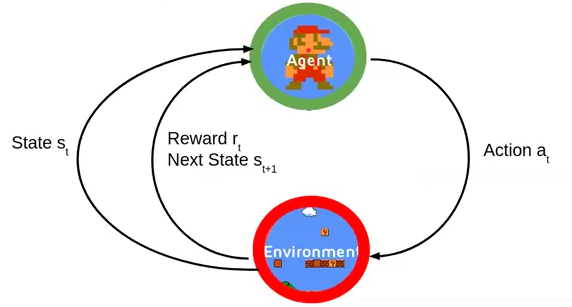
\includegraphics[width=.75\textwidth]{090}
    \caption{Reinforcement Learning Loop example of the Mario game.}
    \label{fig:090}
\end{figure}

Agent can take actions that affect the state of the environment and observe occasional rewards that depend on the state. The goal is to learn a \textbf{policy} to maximize the expected reward over time, where a \emph{policy} is a mapping from states to actions.

\begin{example}[Reinforcement Learning in Atari Games]
    Let's consider for example the Atari games. We can perform reinforcement learning with the following assumption:
    \begin{itemize}[topsep={0pt}, partopsep={0pt}]
        \itemsep0pt
        \item The \textbf{objective} is to complete the game with the highest score.
        \item The \textbf{state} are the raw pixel inputs of the game state.
        \item The \textbf{actions} are the game controls (e.g. left, righ, up and down).
        \item The \textbf{reward} is the score, that increases or decreases at each time step.
    \end{itemize}
\end{example}

\section{Markov Decision Process}
The \textbf{Markov Decision Process (MDP)} is a framework used to hep to make decisions on a stochastic environment. It provides a mathematical framework for modeling decision making in situations where outcomes are partly random and partly under the control of a decision maker. Our goal is to find a policy, which is a map that gives us all optimal actions on each state in our environment. In order to solve MDPs we need Dynamic Programming (DP), more specifically the \textbf{Bellman equation}. 

Recall that Dynamic Programming is a method that divides a problem into simple sub-problems easier to solve, but, differently from the divide and conquer method, it stores the results that are repeated in a table, in order to make the algorithm more efficient.

At each time step, the process is in some state \(s\), and the decision maker may choose any action \(a\) that is available in state \(s\). The process responds at the next time step by randomly moving into a new state \(s'\), and giving the decision make a corresponding reward \(R_a(s,s')\).

The probability that the process moves into its new state \(s'\) is influenced by the chosen action. Specifically, it is given by the state transaction function \(P_a(s,s')\). Thus, the next state \(s'\) depends on the current state \(s\) and the decision maker's action \(a\). But given \(s\) and \(a\), it is \emph{conditionally independent} of all previous states and actions.

\begin{figure}[t!]
    \centering
    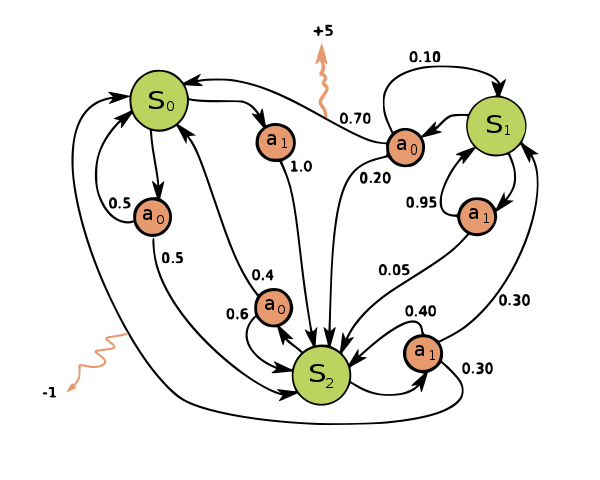
\includegraphics[width=.75\textwidth]{091}
    \caption{Example of a simple MDP with three states (big circles) and two actions (small circles), with two rewards (waved arrows).}
    \label{fig:091}
\end{figure}

\subsection{Definition}
A Markov decision process is a 5-tuple \((\mathcal{S}, \mathcal{A}, \mathcal{R}, P, \gamma)\), where:
\begin{itemize}[topsep={0pt}, partopsep={0pt}]
    \itemsep0pt
    \item \(\mathcal{S}\) is a set of states called the \textbf{state space},
    \item \(\mathcal{A}\) is a set of actions called the \textbf{action space}, alternatively \(\mathcal{A}_s\) is the set of actions available from state \(s\),
    \item \(\mathcal{R}_a(s,s')\) is the immediate reward (or expected immediate reward) received after transitioning from state \(s\) to state \(s'\), due to action \(a\),
    \item \(P_a(s,s') = Pr(s_{t+1}=s' | s_t=s, a_t=a)\) is the probability that action \(a\) in state \(s\) at time \(t\) will lead to state \(s'\) at time \(t+1\),
    \item \(\gamma\) is the discount factor. 
\end{itemize}
A policy function \(\pi\) is a (potentially probabilistic) mapping from state space \(\mathcal{S}\) to an action space \(\mathcal{A}\).

\subsection{MDP Loop}
At time step \(t=0\), the environment samples the initial state \(s_0 \sim p(s_0)\). From that initialization, starts the loop, repeat the following steps:
\begin{itemize}
    \item Agent selects action \(a_t\);
    \item Environment samples reward \(r_t \sim \mathcal{R}( \cdot | s_t, a_t)\),
    \item Environment samples the next state \(s_{t+1} \sim P( \cdot | s_t, a_t)\),
    \item Agent receives reward \(r_t\) and next state \(s_{t+1}\).
\end{itemize}

\subsection{Objective}
The goal in Marvok Decision Process is to find a good policy for the decision maker: a function \(pi\) that specifies the action \(\pi(s)\) that the decision maker will choose when in state \(s\). Once a MDP is combined with a policy in this way, this fixes the action for each state.

The objective is to choose a policy \(\pi\) that will maximize some cumulative function of the random rewards. A policy that maximizes the cumulative discounted reward is called an optimal policy \(\pi^*\).

\subsubsection{Cumulative Discounted Rewards}
Suppose the following policy \(\pi\) starting in state \(s_0\) leads to a sequence \(s_0, s_1, s_2, ...\)

The cumulative reward of the sequence is:
\begin{equation}
    \sum_{t \geq 0} r(s_t)
\end{equation}
State sequences can vary in length or een be infinite. Typically we define the cumulative reward as sum of rewards discounted by a factor \(\gamma\):
\begin{align}
    r(s_0) + \gamma r(s_1) + \gamma^2 r(s_2) + \gamma^3 r(s_3) + ... = \\
    = \sum_{t \geq 0} \gamma^t r(s_t), \qquad 0 < \gamma \leq 1
\end{align}
The discounting factor \(\gamma\) controls the importance of the future rewards versus the immediate ones. The lower the discount factor is, the less important future rewards are, and the agent will tend to focus on actions which will yield immediate rewards only. The cumulative reward is bounded, and this helps the algorithm to converge.

\subsection{Reinforcement Learning vs Supervised Learning}
In supervised learning, the loop follows these steps:
\begin{itemize}
    \item Get input \(x_i\) samples from data distribution.
    \item Use model with parameters \(w\) to predict output \(y\).
    \item Observe target output \(y_i\) and loss \(l(w,x_i,y_i)\).
    \item Update \(w\) to reduce loss with SGD:
    \begin{equation}
        w \gets w - \eta \nabla l (w, x_i, y_i)
    \end{equation}
\end{itemize}
While, as we have seen, the reinforcement learning loop follows these steps:
\begin{itemize}
    \item From state \(s\), take action \(a\) determined by policy \(\pi(s)\).
    \item Environment selects next state \(s'\) based on transition model \(P(s' | s,a)\).
    \item Observe \(s'\) and reward \(r(s)\), then update the policy.
\end{itemize}

In Supervised learning the next input does not depend on the previous inputs or agent predictions, there is a supervision signal at every step, and the loss is differentiable with respect to model parameters. 

In reinforcement learning agent's actions affect the environment and help to determine the next observation, the rewards may be sparse and are not differentiable with respect to model parameters.

\section{Value Based Methods}
The \textbf{value function} gives the total amount of reward the agent can expect from a particular state to all possible states from that state. With the value function you can find a policy. The value function \(V\) of a state \(s\) with respect to policy \(\pi\) is hte expected cumulative reward of following that policy starting in \(s\):
\begin{equation}
    V^\pi (s) = \mathbb{E} \left[
        \sum_{t \geq 0} \gamma^t r(s_t) | s_0 = s, \pi
    \right]
\end{equation}
with \(a_t = \pi(s_t), s_{t+1} \sim P( \cdot | s_t, a_t)\).

The \textbf{optimal value of a state} is the value achievable by ollowing the best possible policy:
\begin{equation}
    V^*(s) = \max_\pi \mathbb{E} \left[
        \sum_{t \geq 0} \gamma^t r(s_t) | s_0 = s, \pi
    \right]
\end{equation}

\subsection{\(Q\)-Learning}
Q-learning is a model-free reinforcement learning algorithm to learn the value of an action in a particular state. It does not require a model of the environment (hence "model-free"), and it can handle problems with stochastic transitions and rewards without requiring adaptations.

For any finite Markov decision process (FMDP), \(Q\)-learning finds an optimal policy in the sense of maximizing the expected value of the total reward over any and all successive steps, starting from the current state. \(Q\)-learning can identify an optimal action-selection policy for any given FMDP, given infinite exploration time and a partly-random policy. "\(Q\)" refers to the function that the algorithm computes --- the expected rewards for an action taken in a given state.

\subsubsection{\(Q\)-Value Function}
It is more convenient to define the value of a state-action pair, instead of just the state:
\begin{equation}
    Q^\pi (s,a) = \mathbb{E} \left[
        \sum_{t \geq 0} \gamma^t r(s_t) | s_0 = s, a_0 = a, \pi
    \right]
\end{equation}
In this case, the optimal \(Q\)-value function tells how good is a state-action pair:
\begin{equation}
    Q^* (s,a) = \max_\pi \mathbb{E} \left[
        \sum_{t \geq 0} \gamma^t r(s_t) | s_0 = s, a_0 = a, \pi
    \right]
\end{equation}
When the optimal \(Q\)-value is found it is used to compute the optimal policy:
\begin{equation}
    \pi^* (s) = \arg \max_a Q^* (s,a)
\end{equation}
\begin{figure}[h!]
    \centering
    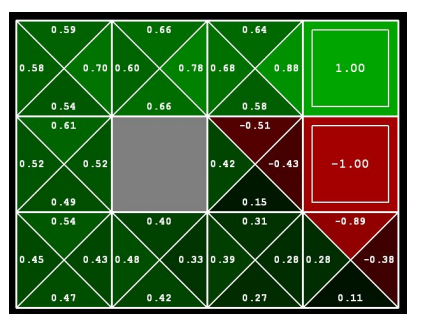
\includegraphics[width=.5\textwidth]{092}
    \caption{Table where we have the maximum expected future reward, for each action at each state.}
    \label{fig:092}
\end{figure}

\subsubsection{Bellman Equation}
The Bellman equation  is a necessary condition for optimality associated with the mathematical optimization method known as dynamic programming.

Recursive relationship between optimal values of successive states and actions:
\begin{align}
    Q^* (s,a) &= r(s) + \gamma \sum_{s'} P(s' | s,a) \max_{a'} Q^* (s',a')\\
    &= \mathbb{E}_{s' \sim P(\cdot | s,a) [ r(s) + \gamma \max_{a'} Q^* (s',a') | s,a]}
\end{align}
If the optimal state-action values for the next time-step \(Q^*(s',a')\) are known, then the optimal strategy is to take the action that maximizes the expected value.

\subsubsection{Algorithm}
After \(\Delta t\) steps into the future, the agent will decide some next step. The weight for this step is calculated as \(\gamma^{\Delta t}\), where \(\gamma\) has the effect of valuing rewards reeiving earlier higher than those received later, it may also be interpreted as the probability to succeed at every step \(\Delta t\).

The algorithm has a funciton that calculates the quality of a state-action combination, that is the \(Q (s,a)\). Before learning begins, \(Q\) is initialized to a possibly arbitrary fixed value. Then, at each time \(t\) the agent selects an action \(a_t\), observes a reward \(r_t\), enters a new state \(s_{t+1}\), and \(Q\) is updated.

As an example, suppose the robot in Figure~\ref{fig:093} needs to reach room 5.
\begin{figure}[h!]
    \centering
    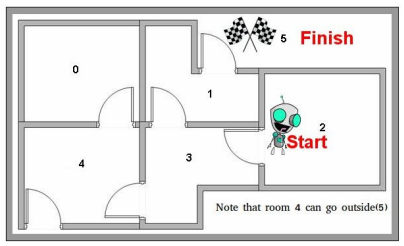
\includegraphics[width=.5\textwidth]{093}
    \caption{We want an agent that is able to find the goal state (5) from the initial state (i.e. 2).}
    \label{fig:093}
\end{figure}
Our components are:
\begin{itemize}
    \item Actions \(\mathcal{A} = \{0,1,2,3,4,5\}\),
    \item States \(\mathcal{S} = \{0,1,2,3,4,5\}\),
    \item Rewards = \{0,100\}.
\end{itemize}
Our goal state is 5. The reward table \(\mathcal{R} = \mathcal{S} \times \mathcal{A}\) is computed based on the possible actions at a certain state, where the value \(-1\) indicate some specific action is not available.
\begin{figure}[h!]
    \centering
    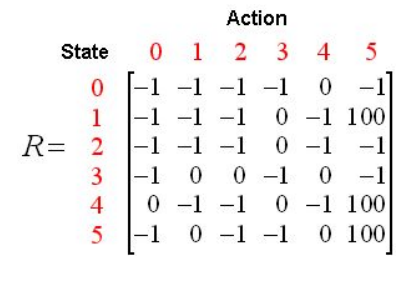
\includegraphics[width=.35\textwidth]{094}
    \caption{}
    \label{fig:094}
\end{figure}
The whole point of \(Q\)-learning is that the matrix \(\mathcal{R}\) is available only to the environment, the agent need to learn \(\mathcal{R}\) by himself through experience.

What the agent will have is a \(Q\) matrix that encodes the state, the action, and the rewards, but is initialized with zero and through experience becomes like the matrix \(\mathcal{R}\). The policy can then be obtained from the \(Q\) matrix.

\begin{algorithm}
    \caption{\(Q\)-Learning}
    \label{alg:q_learning}
    $Q \gets [1...s][1...a] = \{0...0\}\{0...0\}$\;
    $s_0 \gets random$\;
    \For{ episode in $E$ } {
        \While{ state $s_i \neq s_\text{goal}$ }{
            Select a random possible action $a_r$ for $s_i$\;
            Using $a_r$, consider going to this next state\;
            Get maximum \(Q\) value for this next state\;
            $Q^*(s,a) \gets \mathcal{R}(s,a) + \gamma \max_{a'} [Q^* (s',a')]$\;
        }
    }
\end{algorithm}

\subsection{Deep \(Q\)-Learning}
\begin{wrapfigure}{l}{0.25\textwidth}
    \begin{center}
        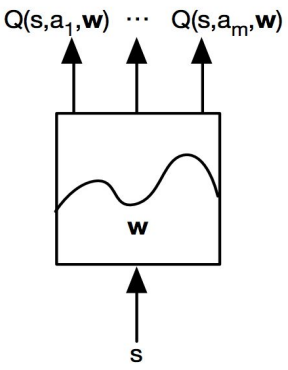
\includegraphics[width=0.25\textwidth]{095}
        \caption{}
    \end{center}
    \label{fig:095}
\end{wrapfigure}
The Bellman equation is a constraint on \(Q\)-values of successive states, the problem is that state spaces for interesting problems are huge (i.e. Atari game), the solution is to approximate \(Q\)-values using a parametric function:
\begin{equation}
    Q^*(s,a) \approx Q_w(s,a)
\end{equation}

We can train a deep network that approximates \(Q\). This is represented in Figure~\ref{fig:095}.

The idea is that, at iteration of training, we can update a the models parameter \(w\) to push \(Q\) close to \(y\):
\begin{equation}
    y_i(s,a) = \mathbb{E}_{s' \sim P( \cdot | s,a)} \left[
        r(s) + \gamma \max_{a'} Q_{w_{i-i}}(s',a') | s,a
    \right]
\end{equation}
The loss function (that change at each iteration) is defined as:
\begin{equation}
    L_i (w_i) = \mathbb{E}_{s, a \sim \rho} \left[
        (y_i(s,a) - Q_{w_i} (s,a))^2
    \right]
\end{equation}
where \(\rho\) is a probability distribution over states \(s\) and actions \(a\) that we refer to as the \textbf{behaviour distribution}.

In practice the gradient update will be:
\begin{align}
    \nabla_{w_i} L(w_i) &= \mathbb{E}_{s, a \sim \rho} \left[
        (y_i(s,a) + Q_{w_i}(s,a) \nabla_{w_i} Q_{w_i} (s,a)
    \right]\\
    &= \mathbb{E}_{s, a \sim \rho, s'} \left[
        (r(s) + \gamma \max_{a'} Q_{w_{i-i}}(s',a') - Q_{w_i} (s,a)) \nabla_{w_i} Q_{w_i} (s,a)
    \right]
\end{align}
SGD training: replace expectation by sampling \textbf{experiences} \((s,a,s')\) using behaviour distribution and transition model.

The training is prone to instability, unlike in supervised learning, the targets themselves are moving, successive experiences are correlated and dependent on the policy, and the policy may change rapidly with slight changes to parameters, leading to drastic change in data distribution.

Solutions to the training instability can be to freeze the target \(Q\) network, or we can use the experience replay, that is a buffer that stores experiences from which we can sample.

\section{Policy Gradient Methods}
Instead of indirectly representing the policy using the \(Q\)-values, it can be more efficient to parametrize \(\pi\) and learn it directly. Especially in large or continuous action spaces the \(Q\)-value function can be very complicated, for example a robot grasping an object has a very high-dimensional state and it is hard to learn exact value of every (state, action) pair.

In this case it is beneficial to learn a function giving the probability distribution over actions from current state:
\begin{equation}
    \pi_\theta (s,a) \approx P(a|s)
\end{equation}
where the parameter \(\theta\) is the parameter of our neural network.

Let's take as an example the pong game: the basic idea is to use a machine learning model that will learn a good policy from playing the game and receiving rewards.
\begin{figure}[t!]
    \centering
    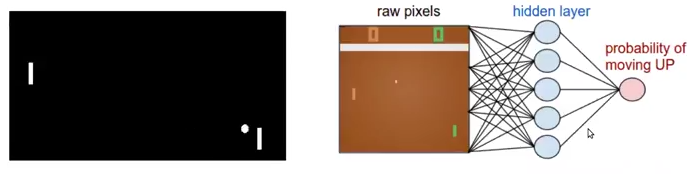
\includegraphics[width=.75\textwidth]{096}
    \caption{Policy Gradient for Pong game.}
    \label{fig:096}
\end{figure}

\subsection{Objective Function}
Our objective function needs to find the best parameter \(\theta\) (parameters of the policy) to maximize the expected reward (use gradient descent):
\begin{align}
    J(\theta) &= \mathbb{E} \left[
        \sum_{t \geq 0} \gamma^t r_t | \pi_\theta
    \right]\\
    &= \underbrace{\mathbb{E}_\tau [r(\tau)]}_{\text{Expectation of return over trajectories } \tau = (s_0, a_0, r_0, s_1, a_1, r_1, ...)}\\
    &= \int_\tau r(\tau) p(\tau; \theta) d\tau
\end{align}
where \(p(\tau; \theta)\) is the probability of trajectory \(\tau\) under policy with parameters \(\theta\), and is defined as follows:
\begin{equation}
    p(\tau; \theta) = \prod_{t \geq 0} \pi_\theta (s_t,a_t) P(s_{t+1} | s_t, a_t)
\end{equation}
\subsubsection{Optimization}
We need a convenient way to compute the graident of \(\mathbb{} [r(\tau)]\), in order to do that it turns out that the gradient can be expressed in the following way:
\begin{equation}
    \nabla_\theta J(\theta) = \mathbb{E} [r(\tau) \nabla_\theta \log p(\tau; \theta)]
\end{equation}
Now, we can continue our computations with some rules of the logarithms for the probability of trajectory \(\tau\):
\begin{align}
    p(\tau; \theta) &= \prod_{t \geq 0} \pi_\theta (s_t, a_t) P(s_{t+1} | s_t, a_t)\\
    \log p(\tau ; \theta) &= \sum_{t \geq 0} [\log \pi_\theta (s_t, a_t) + \log P(s_{t+1} | s_t, a_t)]\\
    \nabla_\theta \log p(\tau; \theta) &= \sum_{t \geq 0} \nabla_\theta \log \pi_\theta (s_t, a_t)
\end{align}
In this way we do not need to know any information about the environment dynamics \(p\). We can now compute the gradient of our objective function:
\begin{equation}
    \nabla_\theta (\theta) = \mathbb{E}_\tau \left[
        \left(
            \sum_{t \geq 0} \gamma^t r_t
        \right) \left(
            \sum_{t \geq 0} \nabla_\theta \log \pi_\theta (s_t, a_t)
        \right)
    \right]
\end{equation}
We can compute this expecation by sampling \(N\) trajectories \(\tau_1, ..., \tau_N\):
\begin{equation}
    \nabla_\theta (\theta) \approx \frac 1 N \sum_{i=1}^N \left(
        \sum_{t = 0}^{T_i} \gamma^t r_{i,t}
    \right) \left(
        \sum_{t = 0}^{T_i} \nabla_\theta \log \pi_\theta (s_{i,t}, a_{i,t})
    \right)
\end{equation}
\subsection{Reinforce Algorithm}
This leads to the \textbf{reinforce algorithm}, the intuition behind that is that if we are going up the hill it means that we are receiving an higher reward, we will change the model parameters and thus the policy to increase the likelihood of trajectories that move higher. A representation of that can be found in Figure~\ref{fig:097}
\begin{figure}[t!]
    \centering
    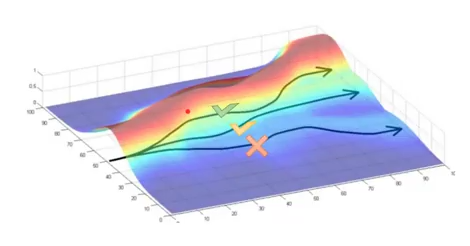
\includegraphics[width=.5\textwidth]{097}
    \caption{}
    \label{fig:097}
\end{figure}

\begin{algorithm}
    \caption{Reinforce}
    \label{alg:reinforce}
    
    Sample \(N\) trajectories \(\tau_i\) using current policy \(\pi_\theta\)\;
    Estimate the policy gradient:
    \begin{equation}
        \nabla_\theta J (\theta) \approx \frac 1 N \sum_{i=1}^N r (\tau_i) \left(
            \sum_{t=0}^{T_i} \nabla_\theta \log \pi_\theta (s_{i,t}, a_{i,t})
        \right)
    \end{equation}
    Update the parameters by gradient ascent:
    \begin{equation}
        \theta \gets \theta + \eta \nabla_\theta J(\theta)
    \end{equation}

\end{algorithm}
